\documentclass{beamer}
\usepackage{ctex, hyperref}
\usepackage[T1]{fontenc}

% other packages
\usepackage{latexsym,amsmath,xcolor,multicol,booktabs,calligra}
\usepackage{graphicx,pstricks,listings,stackengine}

\author{userElaina}
\title{SNN 和 BPTT}
\subtitle{}
\institute{人工智能学院}
\date{2023年08月17日}
\usepackage{JilinUniv}

% defs
\def\cmd#1{\texttt{\color{red}\footnotesize $\backslash$#1}}
\def\env#1{\texttt{\color{blue}\footnotesize #1}}
\definecolor{deepblue}{rgb}{0,0,0.5}
\definecolor{deepred}{rgb}{0.6,0,0}
\definecolor{deepgreen}{rgb}{0,0.5,0}
\definecolor{halfgray}{gray}{0.55}

\lstset{
    basicstyle=\ttfamily\small,
    keywordstyle=\bfseries\color{deepblue},
    emphstyle=\ttfamily\color{deepred},    % Custom highlighting style
    stringstyle=\color{deepgreen},
    numbers=left,
    numberstyle=\small\color{halfgray},
    rulesepcolor=\color{red!20!green!20!blue!20},
    frame=shadowbox,
}


\begin{document}

\kaishu
\begin{frame}
    \titlepage
    \begin{figure}[htpb]
        \begin{center}
            
\includegraphics[width=0.15\linewidth]{pic/Jilin_University_Logo.eps}
        \end{center}
    \end{figure}
\end{frame}

\begin{frame}
    \tableofcontents[sectionstyle=show,subsectionstyle=show/shaded/hide,subsubsectionstyle=show/shaded/hide]
\end{frame}


\section{神经元模型}

\begin{frame}{IF 模型物理推导}
    \begin{equation*}
        \begin{aligned}
            Q(t)
            &= CV(t) \\
            I(t)
            &= I_C(t) \\
            &= \frac{{\rm d}Q}{{\rm d}t} \\
            &= C\frac{{\rm d}V(t)}{{\rm d}t} \\
            RC\frac{{\rm d}V(t)}{{\rm d}t}
            &= RI(t)
        \end{aligned}
    \end{equation*}
\end{frame}

\begin{frame}{IF 模型离散表示推导}
    \begin{equation*}
        \begin{aligned}
            \tau\frac{{\rm d}V(t)}{{\rm d}t}
            &= X(t) \\
            \tau(V_t-V_{t-1})
            &= X_t \\
            V_t
            &= V_{t-1}+\frac{1}{\tau} X_t
        \end{aligned}
    \end{equation*}
\end{frame}

\begin{frame}
    \begin{figure}[l]
        % \centering
        \includegraphics[height=.1\textheight]{pic/lif.jfif}
        \caption{LIF 模型}
    \end{figure}
\end{frame}


\begin{frame}{LIF 模型物理推导}
    \begin{equation*}
        \begin{aligned}
            I_R(t)
            &= \frac{V(t)}{R} \\
            Q(t)
            &= CV(t) \\
            I_C(t)
            &= \frac{{\rm d}Q}{{\rm d}t} \\
            &= C\frac{{\rm d}V(t)}{{\rm d}t} \\
            I(t)
            &= I_R(t)+I_C(t) \\
            &= \frac{V(t)}{R} + C\frac{{\rm d}V(t)}{{\rm d}t} \\
            RC\frac{{\rm d}V(t)}{{\rm d}t}
            &= -V(t) + RI(t)
        \end{aligned}
    \end{equation*}
\end{frame}

\begin{frame}{LIF 模型离散表示推导}
    \begin{equation*}
        \begin{aligned}
            \tau\frac{{\rm d}V(t)}{{\rm d}t}
            &= -V(t)+X(t) \\
            \tau(V_t-V_{t-1})
            &= -V_t+X_t \\
            V_t
            &= (1-\frac{1}{\tau})V_{t-1}+\frac{1}{\tau} X_t
        \end{aligned}
    \end{equation*}
\end{frame}

\section{RNN 的 BPTT 算法}

\begin{frame}
    \begin{figure}[l]
        \centering
        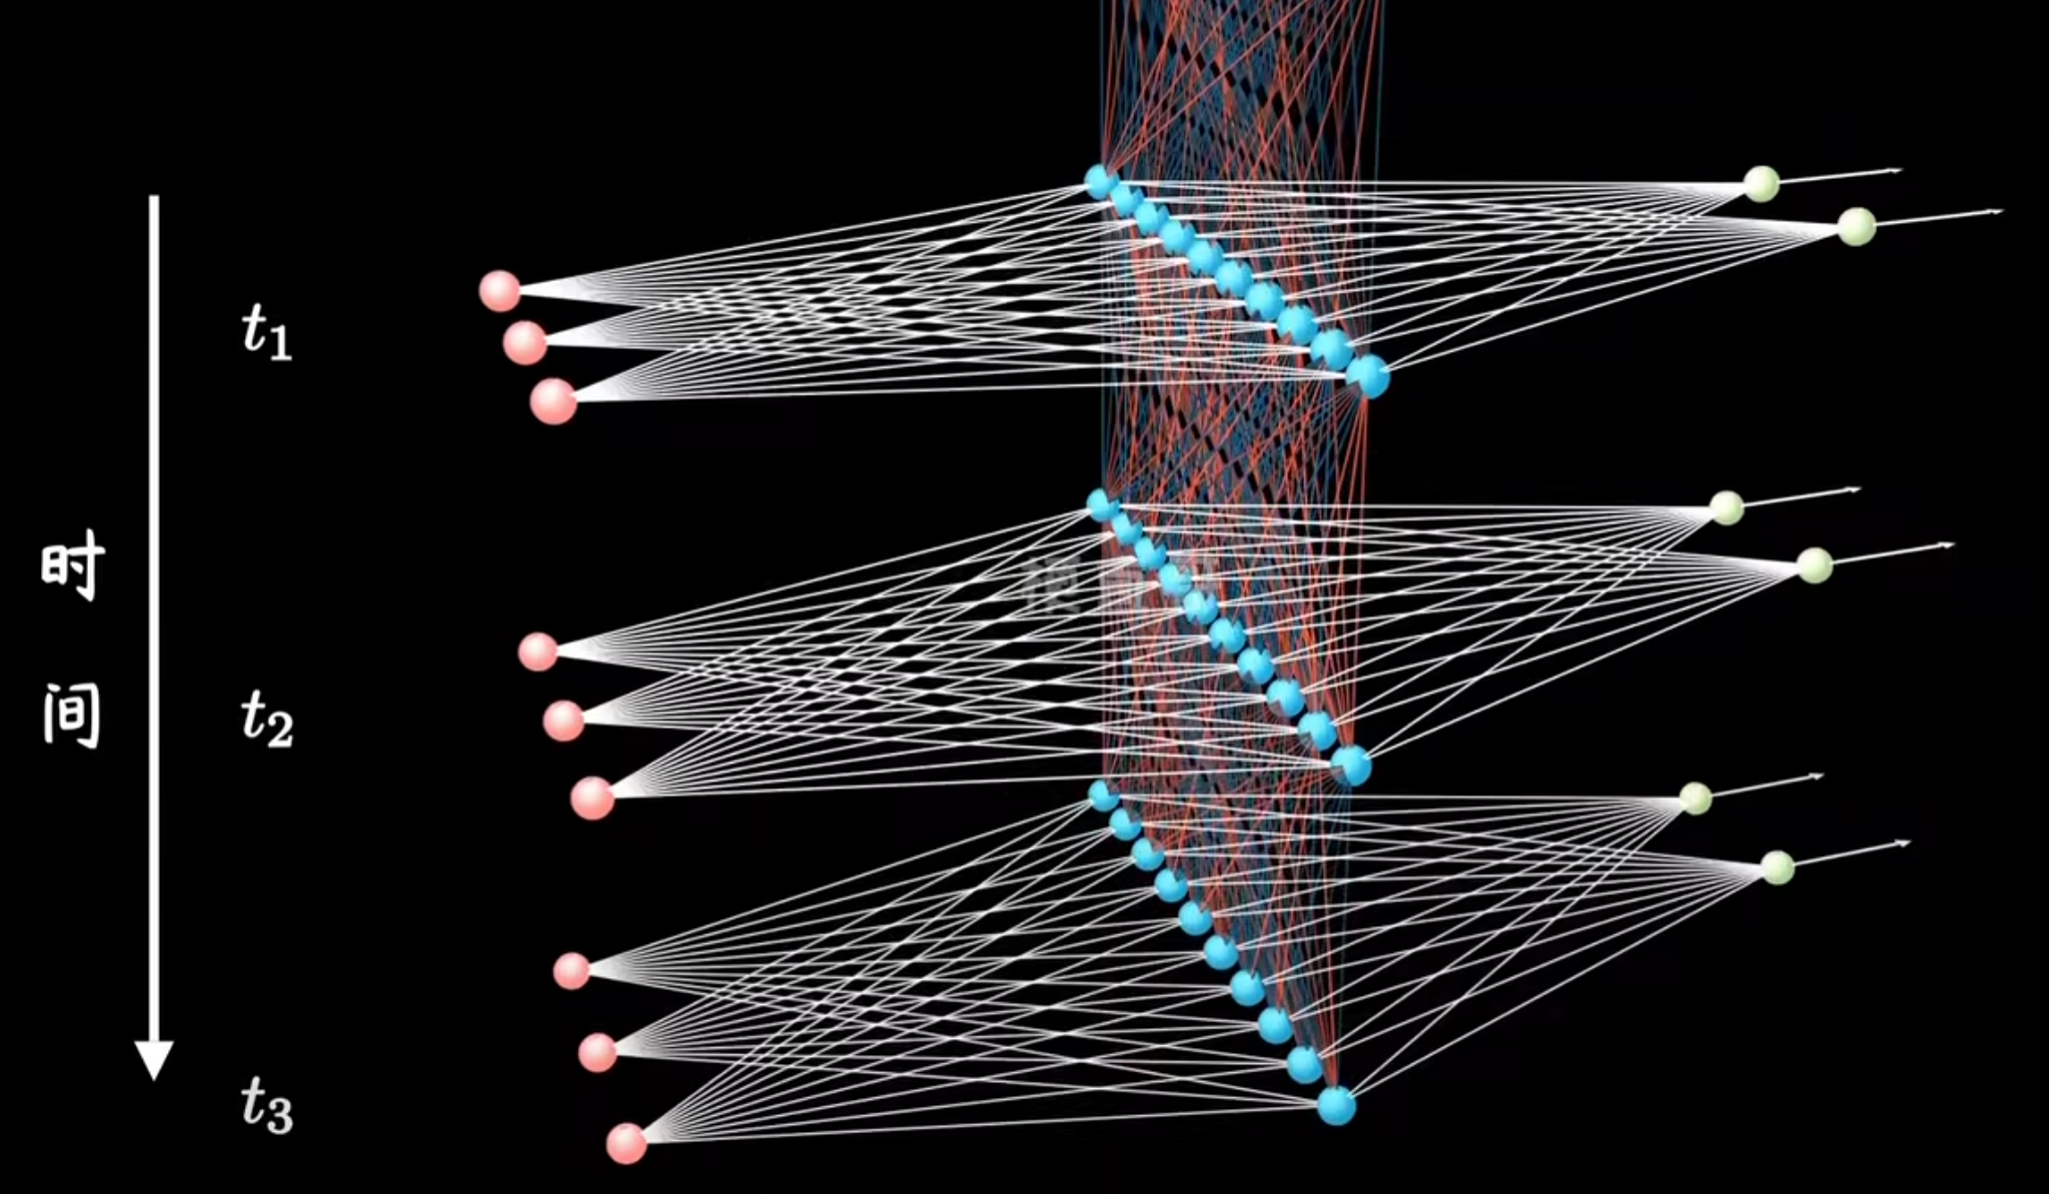
\includegraphics[height=.75\textheight]{pic/rnn.png}
        % \caption{基于粒子群优化的子图匹配插件}
    \end{figure}
\end{frame}

\begin{frame}
    \begin{figure}[l]
        \centering
        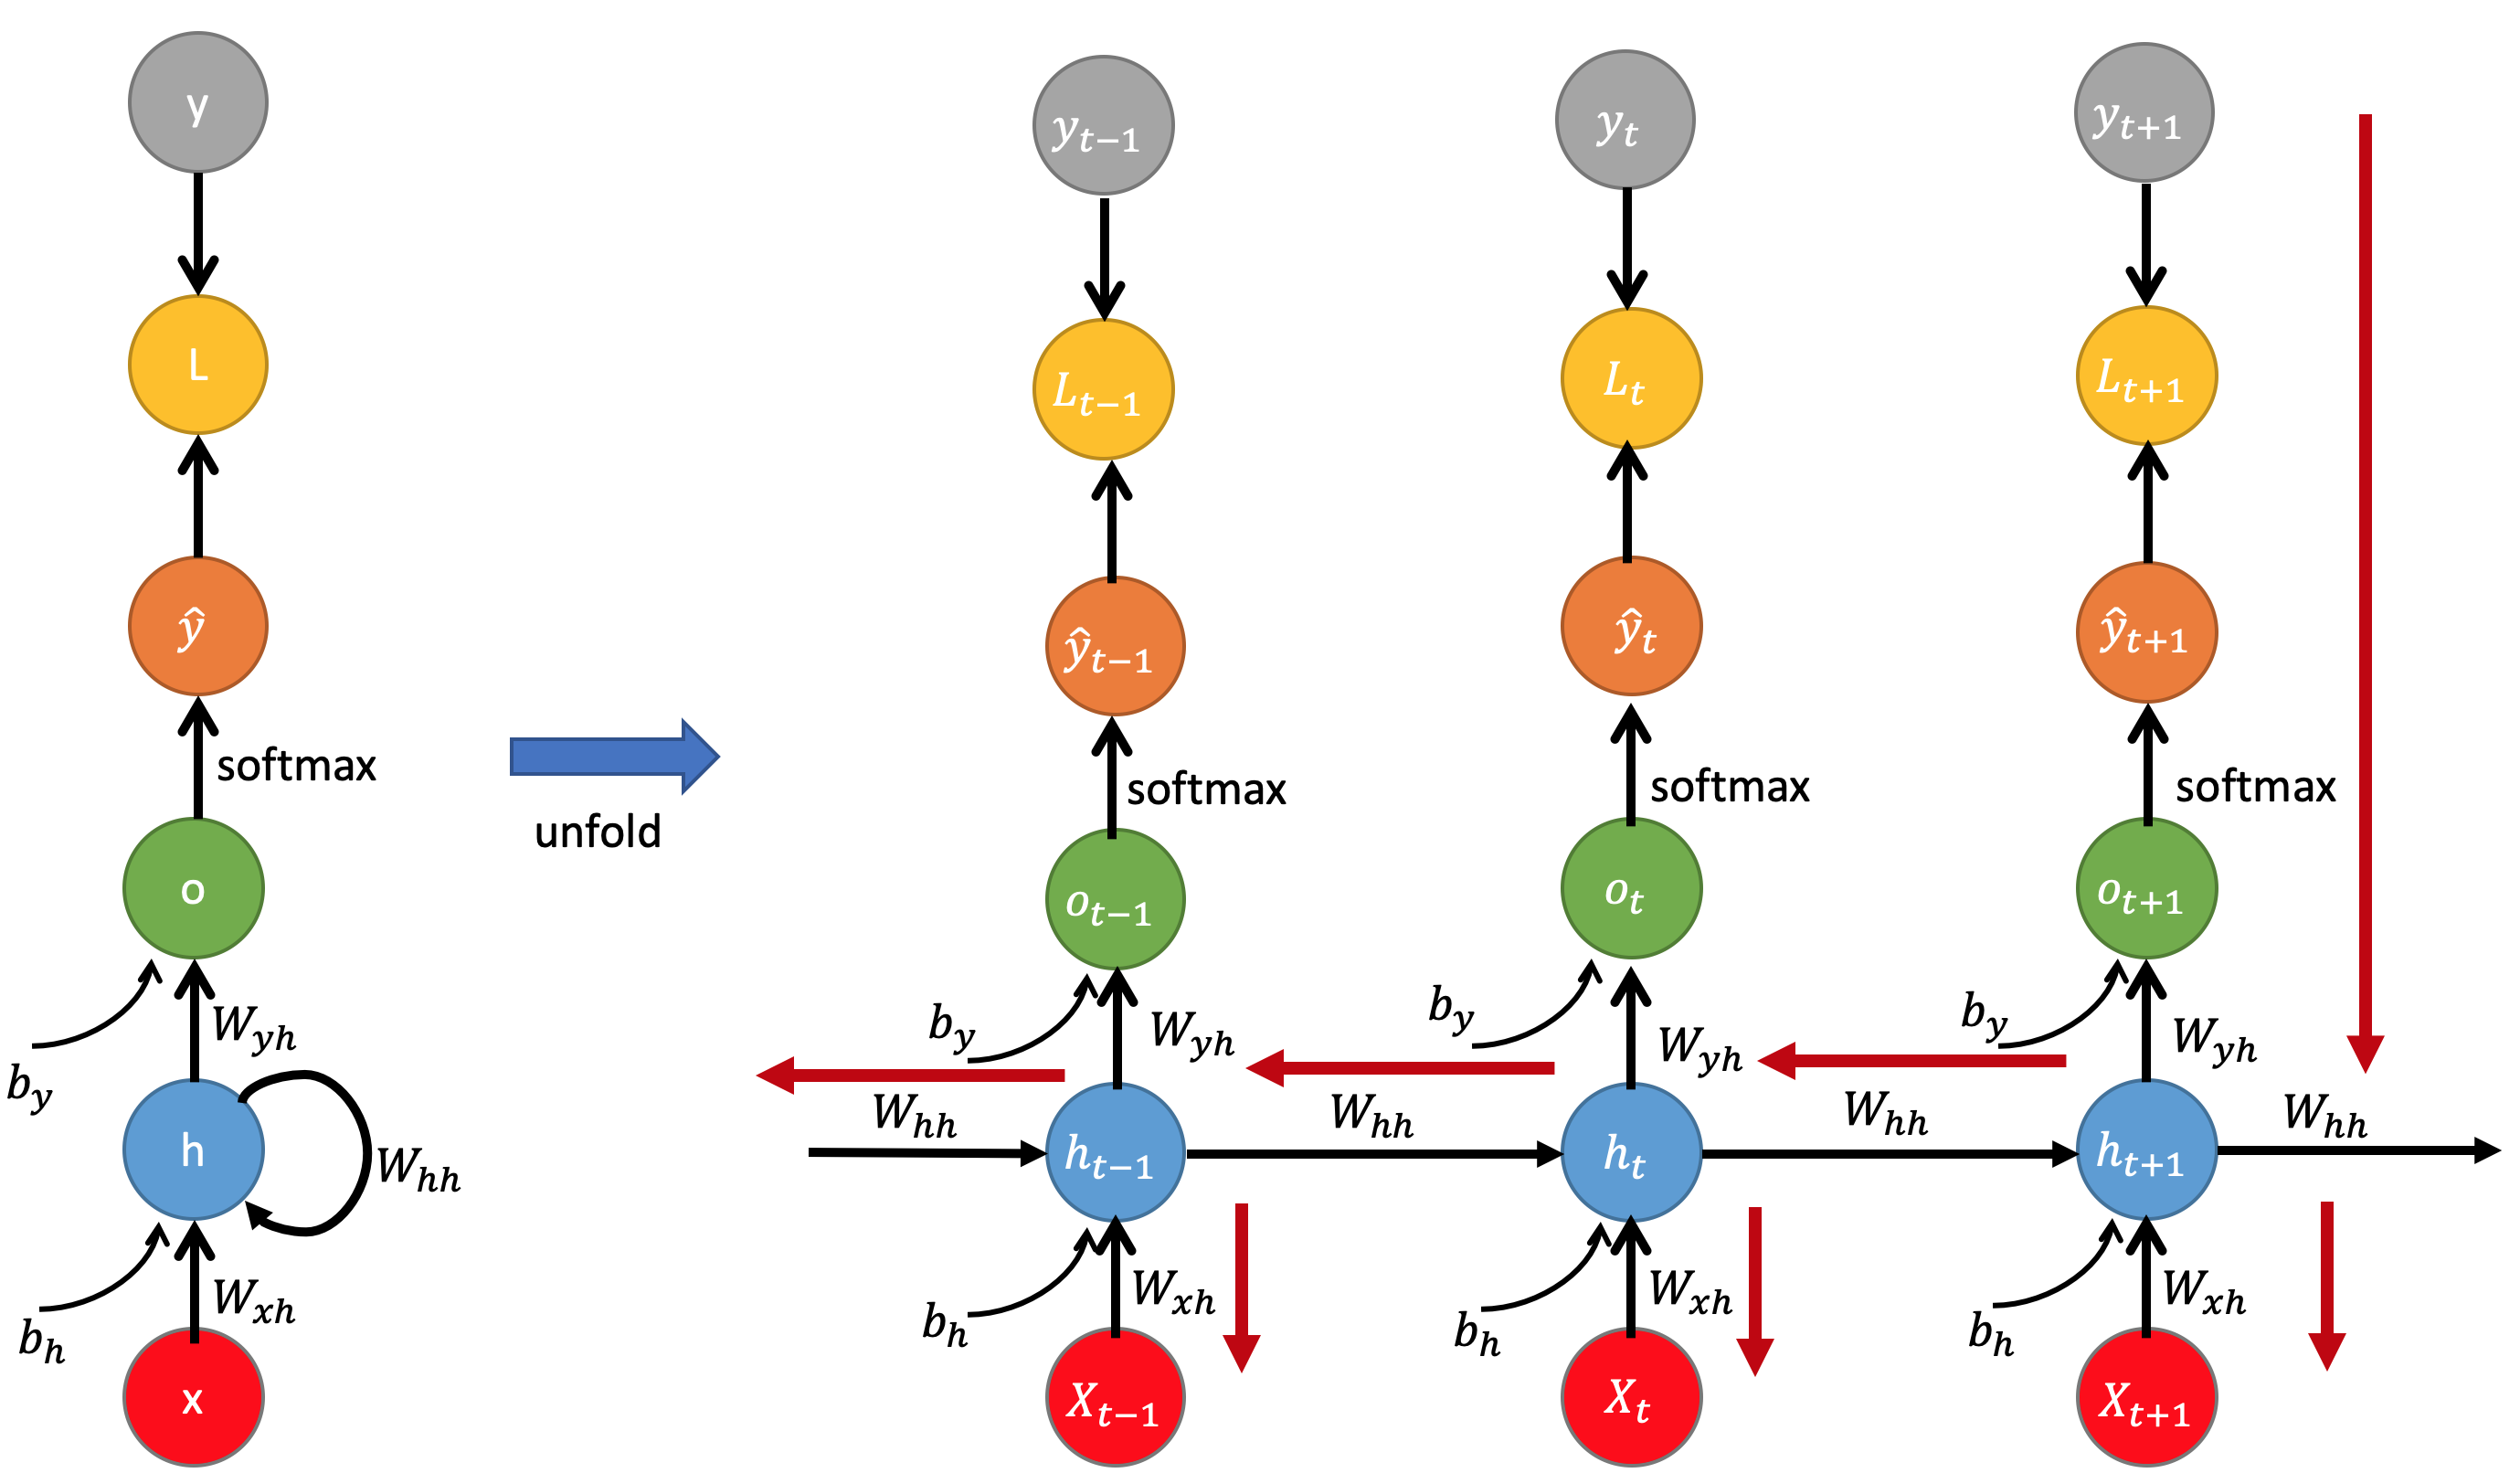
\includegraphics[height=.75\textheight]{pic/bptt.png}
        % \caption{基于粒子群优化的子图匹配插件}
    \end{figure}
\end{frame}


\begin{frame}
    \begin{equation*}
        \begin{aligned}
            h_t &= \Phi_h(X_t\cdot W_{xh}+h_{t−1}\cdot W_{hh}+b_h) \\
            o_t &= h_t\cdot W_{yh}+b_y \\
            \hat{y}_t &= \Phi_o(o_t) \\
            L &= \sum_{i=1}^T L_t \\
            L_t &= -y_t\log\hat{y}_t
        \end{aligned}
    \end{equation*}
\end{frame}

\begin{frame}
    \begin{equation*}
        \begin{aligned}
            \frac{\partial L_t}{\partial b_y}
            &= \frac{\partial L_t}{\partial\hat{y}_t}\frac{\partial\hat{y}_t}{\partial o_t}\frac{\partial o_t}{\partial b_y} \\
            \frac{\partial L_t}{\partial W_{yh}}
            &= \frac{\partial L_t}{\partial\hat{y}_t}\frac{\partial\hat{y}_t}{\partial o_t}\frac{\partial o_t}{\partial W_{yh}}
        \end{aligned}
    \end{equation*}
\end{frame}

\begin{frame}
    \begin{equation*}
        \begin{aligned}
            \frac{\partial L_{t+1}}{\partial W_{hh}}
            &= \frac{\partial L_{t+1}}{\partial\hat{y}_{t+1}}\frac{\partial\hat{y}_{t+1}}{\partial h_{t+1}}\frac{\partial h_{t+1}}{\partial W_{hh}} \\
            &= \frac{\partial L_{t+1}}{\partial\hat{y}_{t+1}}\frac{\partial\hat{y}_{t+1}}{\partial h_{t+1}}\frac{\partial h_{t+1}}{\partial h_t}\frac{\partial h_t}{\partial W_{hh}} \\
            &= \sum_{k=1}^{t+1}\frac{\partial L_{t+1}}{\partial\hat{y}_{t+1}}\frac{\partial\hat{y}_{t+1}}{\partial h_{t+1}}\frac{\partial h_{t+1}}{\partial h_k}\frac{\partial h_k}{\partial W_{hh}} \\
            &= \sum_{k=1}^{t+1}\frac{\partial L_{t+1}}{\partial\hat{y}_{t+1}}\frac{\partial\hat{y}_{t+1}}{\partial h_{t+1}}\left(\Pi_{j=k}^t\frac{\partial h_{j+1}}{\partial h_j}\right)\frac{\partial h_k}{\partial W_{hh}} \\
            \frac{\partial L_{t+1}}{\partial W_{xh}}
            &= \sum_{k=1}^{t+1}\frac{\partial L_{t+1}}{\partial\hat{y}_{t+1}}\frac{\partial\hat{y}_{t+1}}{\partial h_{t+1}}\left(\Pi_{j=k}^t\frac{\partial h_{j+1}}{\partial h_j}\right)\frac{\partial h_k}{\partial W_{xh}} \\
        \end{aligned}
    \end{equation*}
\end{frame}

\begin{frame}
    \begin{equation*}
        \begin{aligned}
            \frac{\partial L}{\partial b_y}
            &= \sum_t^T\frac{\partial L_t}{\partial b_y} \\
            &= \sum_t^T\frac{\partial L_t}{\partial\hat{y}_t}\frac{\partial\hat{y}_t}{\partial o_t}\frac{\partial o_t}{\partial b_y} \\
            \frac{\partial L}{\partial W_{yh}}
            &= \sum_t^T\frac{\partial L_t}{\partial W_{yh}} \\
            &= \sum_t^T\frac{\partial L_t}{\partial\hat{y}_t}\frac{\partial\hat{y}_t}{\partial o_t}\frac{\partial o_t}{\partial W_{yh}} \\
        \end{aligned}
    \end{equation*}
\end{frame}

\begin{frame}
    \begin{equation*}
        \begin{aligned}
            \frac{\partial L}{\partial W_{hh}}
            &= \sum_t^T\frac{\partial L_{t+1}}{\partial W_{hh}} \\
            &= \sum_t^T\sum_{k=1}^{t+1}\frac{\partial L_{t+1}}{\partial\hat{y}_{t+1}}\frac{\partial\hat{y}_{t+1}}{\partial h_{t+1}}\left(\Pi_{j=k}^t\frac{\partial h_{j+1}}{\partial h_j}\right)\frac{\partial h_k}{\partial W_{hh}} \\
            \frac{\partial L}{\partial W_{xh}}
            &= \sum_t^T\frac{\partial L_{t+1}}{\partial W_{xh}} \\
            &= \sum_t^T\sum_{k=1}^{t+1}\frac{\partial L_{t+1}}{\partial\hat{y}_{t+1}}\frac{\partial\hat{y}_{t+1}}{\partial h_{t+1}}\left(\Pi_{j=k}^t\frac{\partial h_{j+1}}{\partial h_j}\right)\frac{\partial h_k}{\partial W_{xh}} \\
        \end{aligned}
    \end{equation*}
\end{frame}

\section{STBP}

\begin{frame}{前向传播}
    \begin{equation*}
        \begin{aligned}
            x_i^{t+1,n} &= \sum_{j=1}^{l(n-1)}w_{ij}^no_j^{t+1,n-1} \\
            u_i^{t+1,n} &= u_i^{t,n}f(o_i^{t,b})+x_i^{t+1,n}+b_i^n \\
            o_i^{t+1,n} &= g(u_i^{t+1,n}) \\
            f(x) &= \tau e^{-\frac{x}{\tau}} \\
            g(x) &= \left\{
                \begin{aligned}
                    1, x &\geq V_{th} \\
                    0, x &< V_{th}
                \end{aligned}
            \right.
        \end{aligned}
    \end{equation*}
\end{frame}

\begin{frame}{反向传播}
    \begin{itemize}
        \item Loss: MSE.
            \begin{equation*}
                \begin{aligned}
                    L=\frac{1}{2S}\sum_{s=1}^S\|y_s-\frac{1}{T}\sum_{t=1}^To_s^{t,N}\|_2^2
                \end{aligned}
            \end{equation*}
        \item 分四种情况讨论 $o$ 和 $u$ 的梯度.
        \item $g$ 不可微. 近似表达脉冲梯度.
    \end{itemize}
\end{frame}

% \begin{frame}
%     \begin{center}
%         {\Huge\calligra Thanks!}
%     \end{center}
% \end{frame}

\end{document}